\chapter{Especificación de requisitos}

Este capítulo es una Especificación de Requisitos Software para el software que se va a realizar siguiendo las directrices dadas por el estándar IEEE830 \cite{iee830}.

\section{Introducción}

\subsection{Propósito}

Este capítulo de especificación de requisitos tiene como objetivo definir las especificaciones funcionales y no funcionales para el desarrollo de un software que permitirá pre-procesar datos DICOM obtenidos al someter a una escultura de madera policromada a una TC para que posteriormente los usuarios puedan realizar labores de documentación al explorar la figura así como realizar una segmentación de los distintos trozos de madera que la componen. 

\subsection{Ámbito del sistema}

En la actualidad, los datos DICOM obtenidos tras una TC se utilizan, principalmente, en el campo donde surgieron, la medicina. Con este software llamado 3DCurator, se tratará de trasladar esta técnica al campo de la restauración de bienes culturales y poder pre-procesar, visualizar, interactuar y documentar los datos DICOM obtenidos con esculturas de madera policromada.

\subsection{Definiciones, acrónimos y abreviaturas}

\begin{itemize}
	\item \textbf{ERS} (Especificación de Requisitos Software).
	\item \textbf{GUI} (Interfaz Gráfica de usuario).
	\item \textbf{\textit{Widget}}: Elemento de la GUI.
	\item \textbf{DICOM} (\textit{Digital Imaging and Communication in Medicine}): Formato de datos volumétricos donde se obtienen las imágenes.
	\item \textbf{CT o TC} (Tomografía Computarizada): Técnica de extracción de datos volumétricos que utiliza radiación X para obtener cortes de objetos.
	\item \textbf{MRI o IRM} (Imagen por Resonancia Magnética): Técnica de extracción de datos volumétricos que utiliza el fenómeno de resonancia magnética nuclear.
	\item \textbf{PET} (Tomografía por Emisión de Positrones): Técnica de extracción de datos volumétricos capaz de medir la actividad metabólica del cuerpo humano.
	\item \textbf{CPU} (\textit{Central Processor Unit}): Microprocesador.
	\item \textbf{GPU} (\textit{Graphic Processor Unit}): Tarjeta gráfica.
	\item \textbf{UML} (Lenguaje unificado de modelado): Lenguaje de modelado de sistemas software.
	\item \textbf{Historia de usuario}: Representación de un requisito utilizando el lenguaje común del usuario.
	\item \textbf{\textit{Product Backlog}}: Listado de historias de usuario del proyecto.
	\item \textbf{C++}: Lenguaje de programación que se usará.
	\item \textbf{XML} (\textit{Extension Markup Language}): Meta lenguaje que se usará para exportar ficheros que después podrán ser importados.
	\item \textbf{CMake} (\textit{Cross platform Make}): Herramienta para generar código compilable en distintas plataformas.
	\item \textbf{Qt}: Librería que se utilizará para realizar la GUI.
	\item \textbf{VTK} (\textit{The Visualization ToolKit}): Librería gráfica que se utilizará para la visualización de volúmenes.
	\item \textbf{ITK} (\textit{Insight Segmentation and Registration Toolkit}): Librería de procesamiento de imágenes que se utilizará.
	\item \textbf{OpenCV}: Librería de visión por computador que se utilizará.
	\item \textbf{Boost}: Conjunto de algoritmos para C++ de los que se usarán la gestión de ficheros XML.
	\item \textbf{Volumen}: Conjunto de datos en los que para cada posición XYZ se tiene un valor determinado.
	\item \textbf{\textit{Voxel}} (\textit{Volumentric Pixel}): Celda en la matriz 3D del conjunto de datos del volumen.
	\item \textbf{Vecinadario}: Celdas alrededor de un voxel.
	\item \textbf{Adyacencia de voxels}: Voxels vecinos que satisfacen un criterio de similitud.
	\item \textbf{Conectividad de voxels}: Voxels entre los cuales hay un camino de voxels adyacentes.
	\item \textbf{Malla}: Estructura de datos con la información de una superficie tridimensional.
	\item \textbf{STL} (\textit{Standard Triangle Language}): Formato que define mallas 3D.
	\item \textbf{Corte}: Vista de la figura a través de un plano. Por ejemplo, al cortar con una sierra un tronco por la mitad, se puede ver cómo es por dentro en esa posición por donde se ha cortado.
	\item \textbf{TF} (Función de transferencia): Función utilizada para visualizar los datos deseados de un volumen.
	\item \textbf{\textit{Preset}}: Función de transferencia previamente configurada.
	\item \textbf{\textit{Direct Volume Rendering}}: Visualización directa de volúmenes en la que cada valor del volumen se mapea con un determinado color y opacidad dado por una función de transferencia.
	\item \textbf{\textit{Ray Casting}}: Técnica de \textit{Direct Volume Rendering} utilizada para la visualización de volúmenes.
	\item \textbf{\textit{Marching Cubes}}: Técnica para generar malla de polígonos a partir de un volumen y un valor de isosuperficie.
	\item \textbf{HU} (\textit{Hounsfield Units}): Unidad de medida escalar del valor de densidad en un \textit{voxel} del volumen.
	\item \textbf{ROD} (\textit{Región de documentación}): Corte en el que se documentará.
	\item \textbf{Regla}: \textit{Widget} utilizado para realizar mediciones de distancias.
	\item \textbf{Transportador de ángulos}: \textit{Widget} utilizado para realizar mediciones de ángulos.
	\item \textbf{Nota}: \textit{Widget} utilizado para realizar anotaciones sobre la figura.
	\item \textbf{Segmentación}: Método por el cual se distinguen distintas partes del volumen.
	\item \textbf{\textit{Thresholding}}: Segmentación basada en umbrales.
	\item \textbf{\textit{Region-growing}}: Segmentación basada en crecimiento de regiones.
	\item \textbf{Semilla}: Coordenada donde se comienza el \textit{region-growing}.
	\item \textbf{\textit{Watershed}}: Técnica de segmentación basada en crecimiento de regiones por inundación.
	\item \textbf{\textit{Canny Edge Detection}}: Algoritmo para resaltar los bordes de una imagen.
	\item \textbf{Transformada de Hough}: Técnica utilizada para detectar líneas rectas.
	\item \textbf{Filtro gaussiano}: Filtro que utiliza la distribución gaussiana del vecindario.
	\item \textbf{Filtro media}: Filtro que utiliza la media del vecindario.
	\item \textbf{Filtro mediana}: Filtro que utiliza la mediana del vecindario.
	\item \textbf{Embón}: Ensamblado de distintos trozos de madera que hacen de base para la escultura.
	\item \textbf{Estuco}: Pasta de grano fino utilizada para realizar correcciones en la escultura.
	\item \textbf{Policromía}: Capa de pintura de las esculturas.
	\item \textbf{Blanco de plomo}: Pigmento de color blanco creado a partir del plomo.
	\item \textbf{Pan de oro}: Lámina muy fina de oro.
\end{itemize}

\subsection{Visión general del documento}

Este capítulo consta de tres secciones:
\begin{itemize}
	\item En la primera sección se realiza una introducción a éste y se proporciona una visión general de la ERS.
	\item En la segunda sección se realiza una descripción general a alto nivel del software, describiendo los factores que afectan al producto y a sus requisitos y con el objetivo de conocer las principales funcionalidades de éste.
	\item En la tercera sección se definen detalladamente los requisitos que deberá satisfacer el software.
\end{itemize}

\section{Descripción general}

\subsection{Perspectiva del producto}

El software 3DCurator tiene como objetivo interactuar con datos DICOM, pero no es el encargado de generarlos. Para generarlos se deberá utilizar algún escáner de TC.

Una vez obtenidos, se podrán pre-procesar aplicando una serie de filtros, segmentar en los distintos trozos de madera que forman la escultura y documentar añadiendo notas y mediciones de distancias y ángulos.

\subsection{Funciones del producto}

Las principales funcionalidades de este sistema serán:

\begin{itemize}
	\item Pre-procesar la imagen aplicando filtros de reducción de ruido:
	\begin{itemize}
		\item Media.
		\item Mediana.
		\item Gaussiano.
	\end{itemize}
	\item Documentar la escultura:
	\begin{itemize}
		\item Agregar anotación.
		\item Agregar regla.
		\item Agregar transportador de ángulos.
	\end{itemize}
	\item Segmentar la escultura por los distintos trozos de madera.
	\item Exportar el volumen.
	\item Importar el volumen.
\end{itemize}

\subsection{Características de los usuarios}

Solo existe un tipo de usuario, que es la persona que desee interactuar con los datos DICOM de una escultura. Esta persona no tiene por qué tener habilidad con un equipo informático, por lo que \myTitle deberá tener una GUI intuitiva y fácil de utilizar.

\subsection{Restricciones}

Se llevará a cabo un desarrollo evolutivo basado en un prototipo funcional sobre un software de visualización de datos volumétricos de esculturas de madera ya existente.

Se programará en C++ usando las librerías VTK para la visualización de gráficos, ITK para el filtrado de imágenes, OpenCV para la visión por computador, Boost para la gestión de ficheros XML y Qt para la GUI.

Al usar estas librerías se contará con restricciones funcionales con las que éstas cuentan que se solventarán  reescribiendo el código que sea posible y necesario. 

Aprovechando que se debe usar CMake para compilar las librerías mencionadas, se utilizará también para generar el proyecto, pues se puede generar código compilable en distintas plataformas.

\subsection{Suposiciones y dependencias}

El software se utilizará para poder interactuar con esculturas de madera por lo que se tendrán en cuenta los materiales con los que están hechas la mayoría de estas (madera, estuco y metal). Si se introducen los datos DICOM de cualquier otra cosa con materiales distintos a los utilizados en las esculturas no se visualizará correctamente. Sin embargo se podrá editar la función de transferencia para su correcta visualización.

La única funcionalidad que se vería afectada sería la segmentación en las distintas piezas de madera que la forman pues usaría como dato el valor escalar en HU de la madera.

\section{Requisitos específicos}

\subsection{Interfaces}

Se adaptará la interfaz actual de 3DCurator para agregar las nuevas funcionalidades (Figura \ref{fig:requisitos/boceto-gui-ppal}):

\begin{itemize}
	\item Se crearán botones para importar y exportar volumen, segmentar y aplicar filtro. Éste último lanzará una ventana modal (Figura \ref{fig:requisitos/boceto-gui-filtro}) donde se seleccionará el filtro y parámetros deseados.
	\item A la derecha se colocará la parte de documentación con la que se podrán agregar y eliminar ROD, reglas, transportadores de ángulos y anotaciones.
\end{itemize}

\begin{figure}[H]
	\centering
	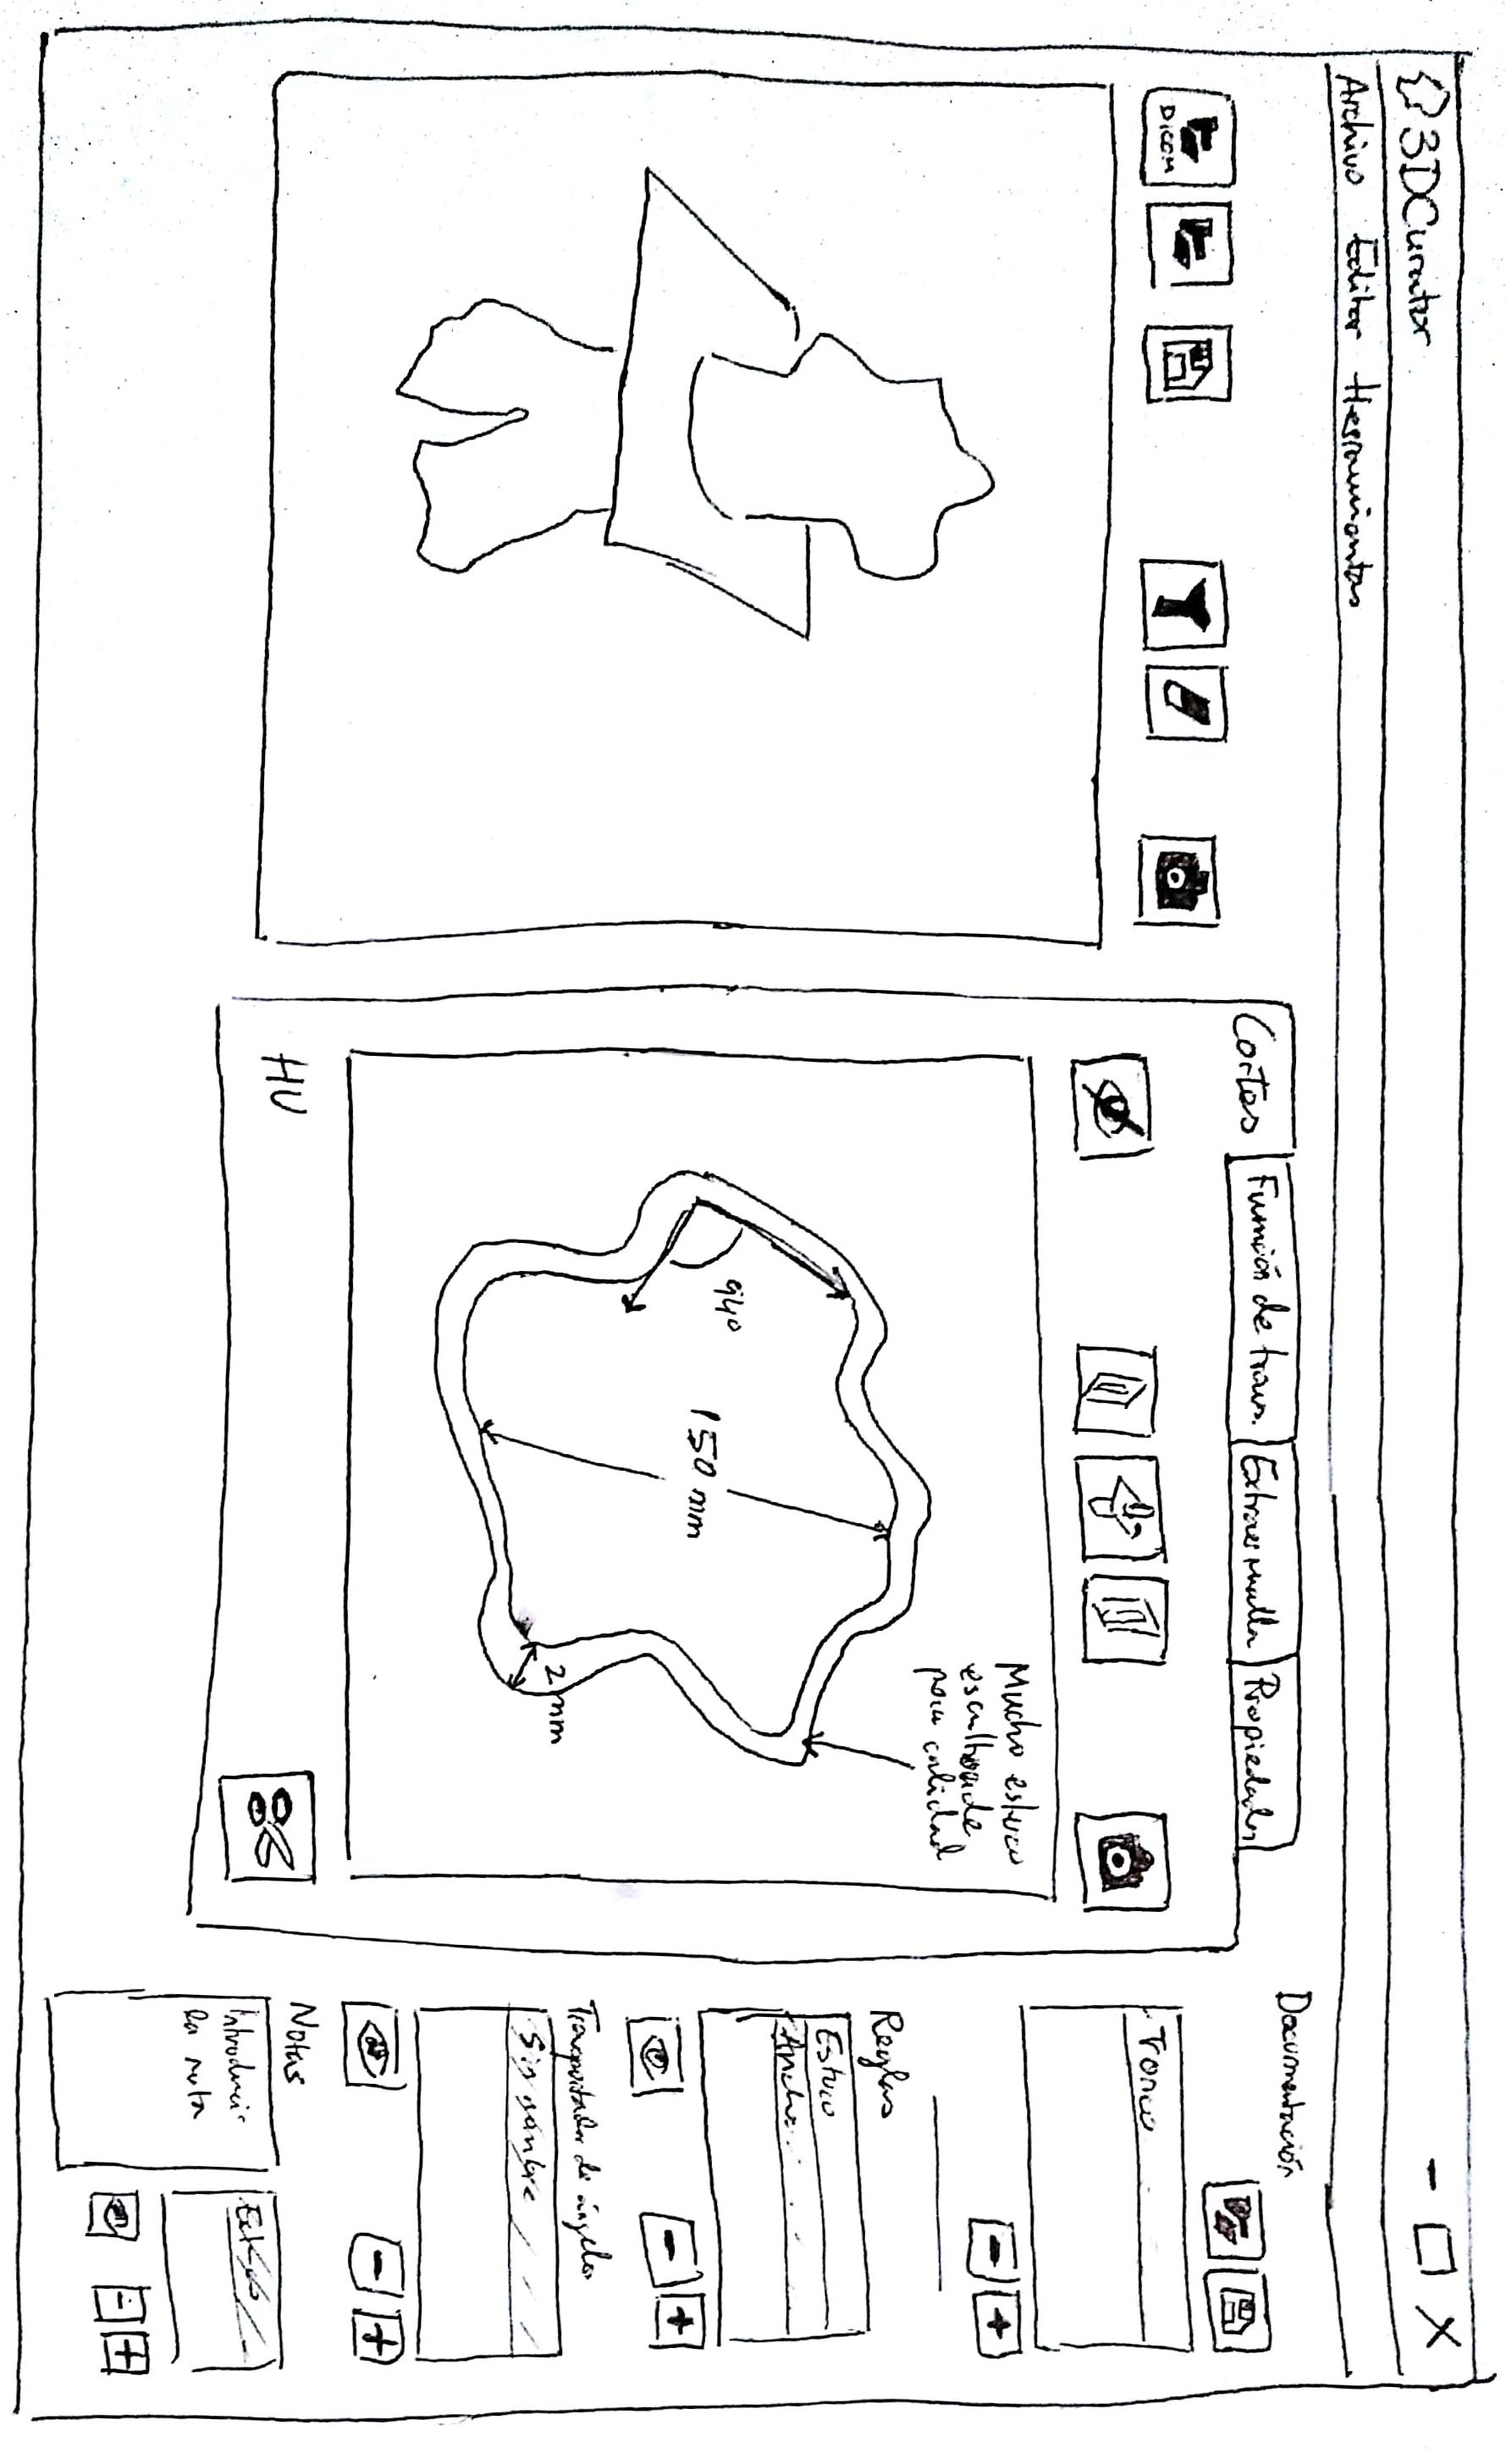
\includegraphics[width=12cm]{imagenes/requisitos/boceto-gui-ppal}
	\caption{Boceto a mano alzada de la posible distribución de los elementos en la GUI principal}
	\label{fig:requisitos/boceto-gui-ppal}
\end{figure}

\begin{figure}[H]
	\centering
	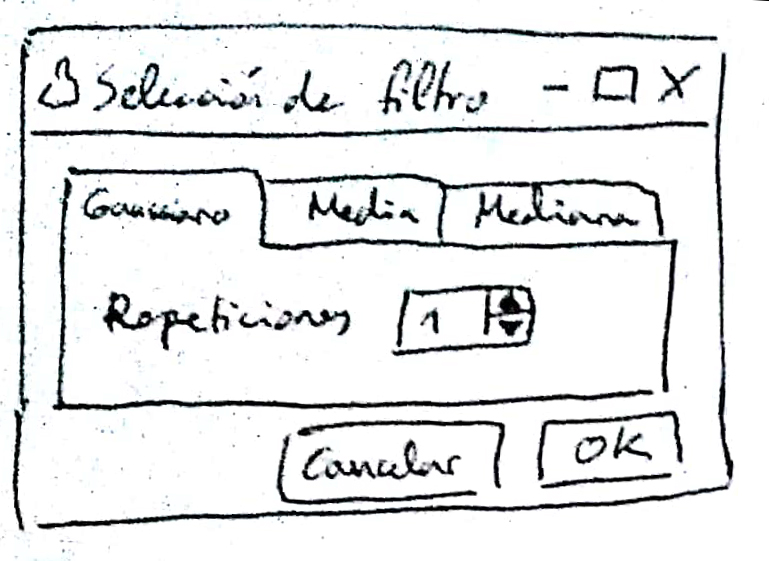
\includegraphics[width=5cm]{imagenes/requisitos/boceto-gui-filtro}
	\caption{Boceto a mano alzada de la posible distribución de los elementos en la GUI de selección de filtros}
	\label{fig:requisitos/boceto-gui-filtro}
\end{figure}

\subsection{Funciones}

El sistema tendrá que realizar distintas funciones que se comentaron anteriormente pero se profundizará en esta sección. Éstas funciones se han estructurado por módulo.

\subsubsection{Auxiliar}

\begin{itemize}
	\item \textbf{Exportar volumen}: El usuario seleccionará la carpeta y el nombre donde deseará guardar el volumen que está visualizando.
	\item \textbf{Importar volumen}: En lugar de cargar directamente los datos DICOM, el usuario podrá cargar el volumen que haya exportado anteriormente el cual puede tener aplicado los filtros de pre-procesamiento o segmentación.
\end{itemize}

\subsubsection{Pre-procesamiento}

\begin{itemize}
	\item \textbf{Filtro gaussiano}: El usuario seleccionará el número de repeticiones que desea aplicar y se aplicará el filtro al volumen cargado.
	\item \textbf{Filtro media}: El usuario seleccionará el tamaño del vecindario y se aplicará el filtro al volumen cargado.
	\item \textbf{Filtro mediana}: El usuario seleccionará el tamaño del vecindario y se aplicará el filtro al volumen cargado.
\end{itemize}

\subsubsection{Segmentación}

\begin{itemize}
	\item \textbf{Segmentar}: Desde un corte, el usuario seleccionará la pieza de madera que desea segmentar. Una vez realizado este proceso se mostrará en pantalla el volumen segmentado y se dará la posibilidad de exportarlo.
\end{itemize}

\subsubsection{Documentación}

\begin{itemize}
	\item \textbf{Crear ROD}: El usuario podrá agregar una ROD a la que podrá dar un nombre.
	\item \textbf{Eliminar ROD}: El usuario podrá eliminar una ROD seleccionada.
	\item \textbf{Exportar ROD}: El usuario podrá exportar la ROD seleccionada.
	\item \textbf{Importar ROD}: El usuario podrá importar una ROD previamente exportada.
	\item \textbf{Cambiar ROD activa}: El usuario podrá cambiar de ROD y se cargará la posición del plano con los elementos de ésta. Si el usuario mueve el plano se dejará de visualizar la ROD actual.
	\item \textbf{Crear regla}: El usuario podrá agregar una regla a la que podrá dar un nombre.
	\item \textbf{Eliminar regla}: El usuario podrá eliminar una regla seleccionada.
	\item \textbf{Ocultar regla}: El usuario podrá ocultar una regla seleccionada.
	\item \textbf{Mostrar regla}: El usuario podrá ocultar una regla seleccionada oculta.
	\item \textbf{Cambiar regla activa}: El usuario podrá cambiar la regla activa.
	\item \textbf{Crear transportador de ángulos}: El usuario podrá agregar un transportador de ángulos al que podrá dar un nombre.
	\item \textbf{Eliminar transportador de ángulos}: El usuario podrá eliminar un transportador de ángulos seleccionado.
	\item \textbf{Ocultar transportador de ángulos}: El usuario podrá ocultar un transportador de ángulos seleccionado.
	\item \textbf{Mostrar transportador de ángulos}: El usuario podrá ocultar un transportador de ángulos seleccionado oculto.
	\item \textbf{Cambiar transportador de ángulos activa}: El usuario podrá cambiar el transportador de ángulos activo.
	\item \textbf{Crear nota}: El usuario podrá agregar una nota a la que podrá dar un nombre y agregar un texto.
	\item \textbf{Eliminar nota}: El usuario podrá eliminar una nota seleccionada.
	\item \textbf{Ocultar nota}: El usuario podrá ocultar una nota seleccionada.
	\item \textbf{Mostrar nota}: El usuario podrá ocultar una nota seleccionada oculta.
	\item \textbf{Cambiar nota activa}: El usuario podrá cambiar la nota activa.
\end{itemize}

\subsection{Requisitos de rendimiento}

Al ser una aplicación de escritorio donde se mostrará y se interactuará con datos, los requisitos de rendimiento no se centrarán en la concurrencia de acceso ni en el almacenamiento, como lo podrían estar en una aplicación web.

Sin embargo, hay que tener en cuenta otros factores, como pueden ser el uso eficiente de memoria y no tener cargadas todos los volúmenes que se han estado visualizando, desechando el anterior cuando se carga uno nuevo.

El rendimiento gráfico también es importante, por eso y para obtener imágenes de mayor calidad, se utilizarán técnicas de DVR como el \textit{ray casting}. Estas técnicas necesitan una gran cantidad de procesamiento, pero la velocidad de procesamiento de las GPU actuales no deberían resultar un problema.

En cuanto a la segmentación que es la función más compleja y costosa computacionalmente, habrá que tener especial cuidado con la gestión de memoria intentando usar los almacenes de datos más adecuados en cada caso.

\subsection{Restricciones de diseño}

Al utilizar librerías como VTK, ITK, OpenCV o Boost, se seguirá la estructura de las mismas a la hora de construir el software, y se tendrán restricciones en cuanto a funcionalidad que se pueda construir con éstas. No obstante son librerías muy completas y no se debería encontrar casi ninguna restricción a excepción de la parte del pre-procesamiento y segmentación donde quizás haya que generar algoritmos propios.

\subsection{Atributos del software}

Al usar CMake, se podrá crear un software multiplataforma que funcione en cualquier sistema operativo.

El software generado deberá ser fiable, porque aunque no trabaje con datos sensibles cuya pérdida pueda ser grave, siempre resulta molesto utilizar un software con fallos que interrumpan una acción durante su uso.

También se debe tener en cuenta que el software sea mantenible pues, en el futuro, otros desarrolladores pueden colaborar y debe estar bien documentado para que esto sea una tarea fácil.

Se tratará de un software de código abierto que se alojará en un repositorio de GitHub.